\chapter{Desenvolvimento}
\label{cap:desenvolvimento}
Este capítulo apresenta o desenvolvimento do sistema responsável pelo processamento de imagens, identificação dos indivíduos e seus tons de pele, detalhando o que cada parte do processo faz e quais parâmetros podem ser alterados para obter-se outros resultados. O processo ocorre em três etapas
distintas. Em um primeiro momento as imagens são inseridas, em seguida é feita a identificação e, finalmente, a classificação.

\begin{figure}[h]
\centering
\caption{Diagrama de desenvolvimento}
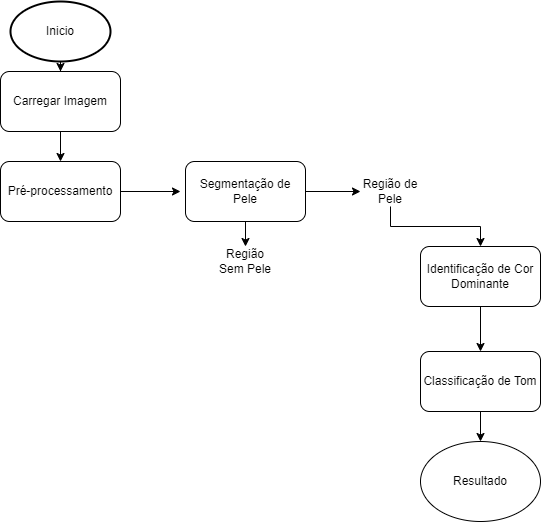
\includegraphics[scale=0.65]{Template_Latex_TCC-UNIFTEC/_lib/imagens/fluxogramaDesenvolvimento.png}

\label{fig: fluxograma_desenvolvimento}
\centering{\Fonte{Autor}}
\end{figure}

A Figura \ref{fig: fluxograma_desenvolvimento} ilustra o processo conceitual básico do sistema proposto para a solução desenvolvida. Para o funcionamento o sistema requer a entrada de uma imagem. A imagem é modificada e convertida para iniciar o pré-processamento. No pré-processamento é executada a identificação da face e regiões a serem excluídas. Em seguida, ocorre a segmentação de pele onde a região de pele e não-pele é separada. Apenas os pixels interpretados como pele são analisados para a identificação de cor dominante e, por fim, a classificação do tom  e saída do resultado com a cor e classificação conforme os tons da paleta de Monk.

Para o desenvolvimento de um sistema para detecção de tom de pele é possível escolher mais de uma região corporal para ser analisada. Contudo, com o objetivo do trabalho mencionado no \ref{cap:introducao}, optou-se pela detecção de face com a pessoa posicionada de frente para a câmera. 

\section{Manipulação de Imagens}
Para a implementação do processo de identificação de tom de pele, foi preciso executar manipulações nas imagens para a realização das etapas de pré-processamento e de resultado visual. Para isso, utilizou-se a biblioteca OpenCV\footnote{https://opencv.org/}. Biblioteca que possui métodos prontos para a manipulação, conversão de imagem e identificação de faces. 

Para o início do processo é preciso a inserção de uma imagem. Para ler as imagens foi utilizado a biblioteca OpenCv com a função imread(). A função imread()\footnote{https://docs.opencv.org/4.x/d4/da8/group\_\_imgcodecs.html\#ga288b8b3da0892bd651fce07b3bbd3a56} carrega uma imagem do arquivo especificado e retorna uma matrix. Além de, ao longo do desenvolvimento foi adicionada a possibilidade de ler imagens utilizando a URL da imagem como entrada com a biblioteca Imutils ao utilizar a função  url\_to\_image() \footnote{https://github.com/PyImageSearch/imutils} e ler uma ou mais imagens a partir de pastas com a função list\_images(). A função url\_to\_image() aceita apenas a URL da imagem. A imagem é baixada e convertida para um array NumPy no formato OpenCV realizando o \textit{download} na memória. A função do list\_images() do módulo paths do Imutils é uma função para localizar imagens recursivamente com base em um diretório raiz. Com isso, foi possível testar uma ou mais imagens por vez na fase de teste relatado no Capítulo \ref{cap:experimentos-resultados}. As três funções permite manipulação de tamanho de imagem, além de permitirem a utilização de vários extensões de arquivo como JPEGs, PNGs, TIFFs e entre outros.

Para a validação da identificação de pele foram utilizadas imagens do \textit{dataset} MST-E\footnote{https://skintone.google/mste-dataset}. O \textit{dataset} possui conjunto de fotos de 19 pessoas com tons de pele distribuídos ao longo da escala de Monk e classificadas pelo Dr. Monk, conforme Figura \ref{fig:x MST_Dataset} totalizando 1515 imagens e 31 vídeos. 

\begin{figure}[h!]
\centering
\caption{Proporção de quantidade de imagens por classificação de cor}
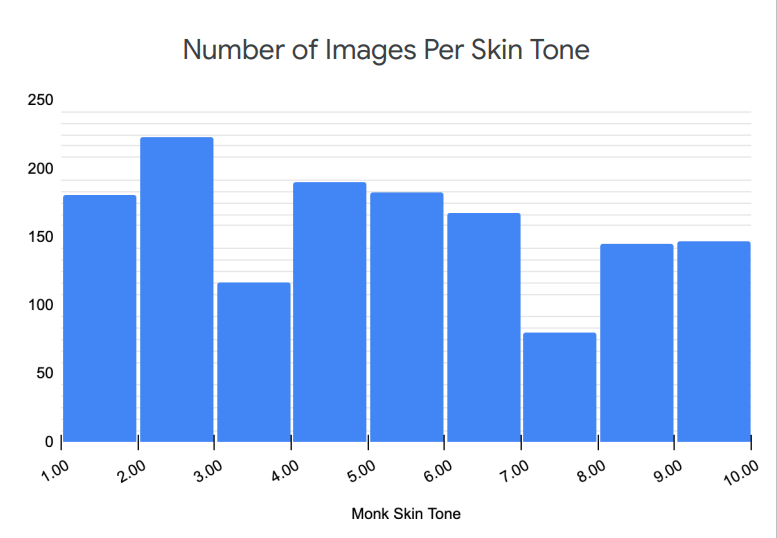
\includegraphics[scale=0.9]{Template_Latex_TCC-UNIFTEC/_lib/imagens/MSTDataset.png}

\label{fig:x MST_Dataset}
\centering{\Fonte{Skin Tone Research} \footnote{https://skintone.google/mste-dataset}}
\end{figure}

Na Figura \ref{fig:x MST_Dataset} demonstra-se a quantidade de imagens por classificação de tom de pele. O conjunto de amostras possui uma distribuição de tons consistentes, contudo os tons 3 e 7 apresentam menos imagens disponíveis. Nota-se que a diferença de quantidade imagens é entorno de 150 imagens entre o tom 2 e 7. Para o trabalho isso não é um impeditivo, pois o \textit{dataset} não é disponibilizado para treinamento de modelo. O \textit{dataset} é utilizada para estudo e verificação dos resultados. Logo, não há interferência no modelo utilizado, apenas dispõe menos exemplos de validação para o tom.


\begin{figure}[h!]
\caption{Exemplos de poses do dataset}
    \label{fig: poses}
    \begin{minipage}[!]{0.55\linewidth}
    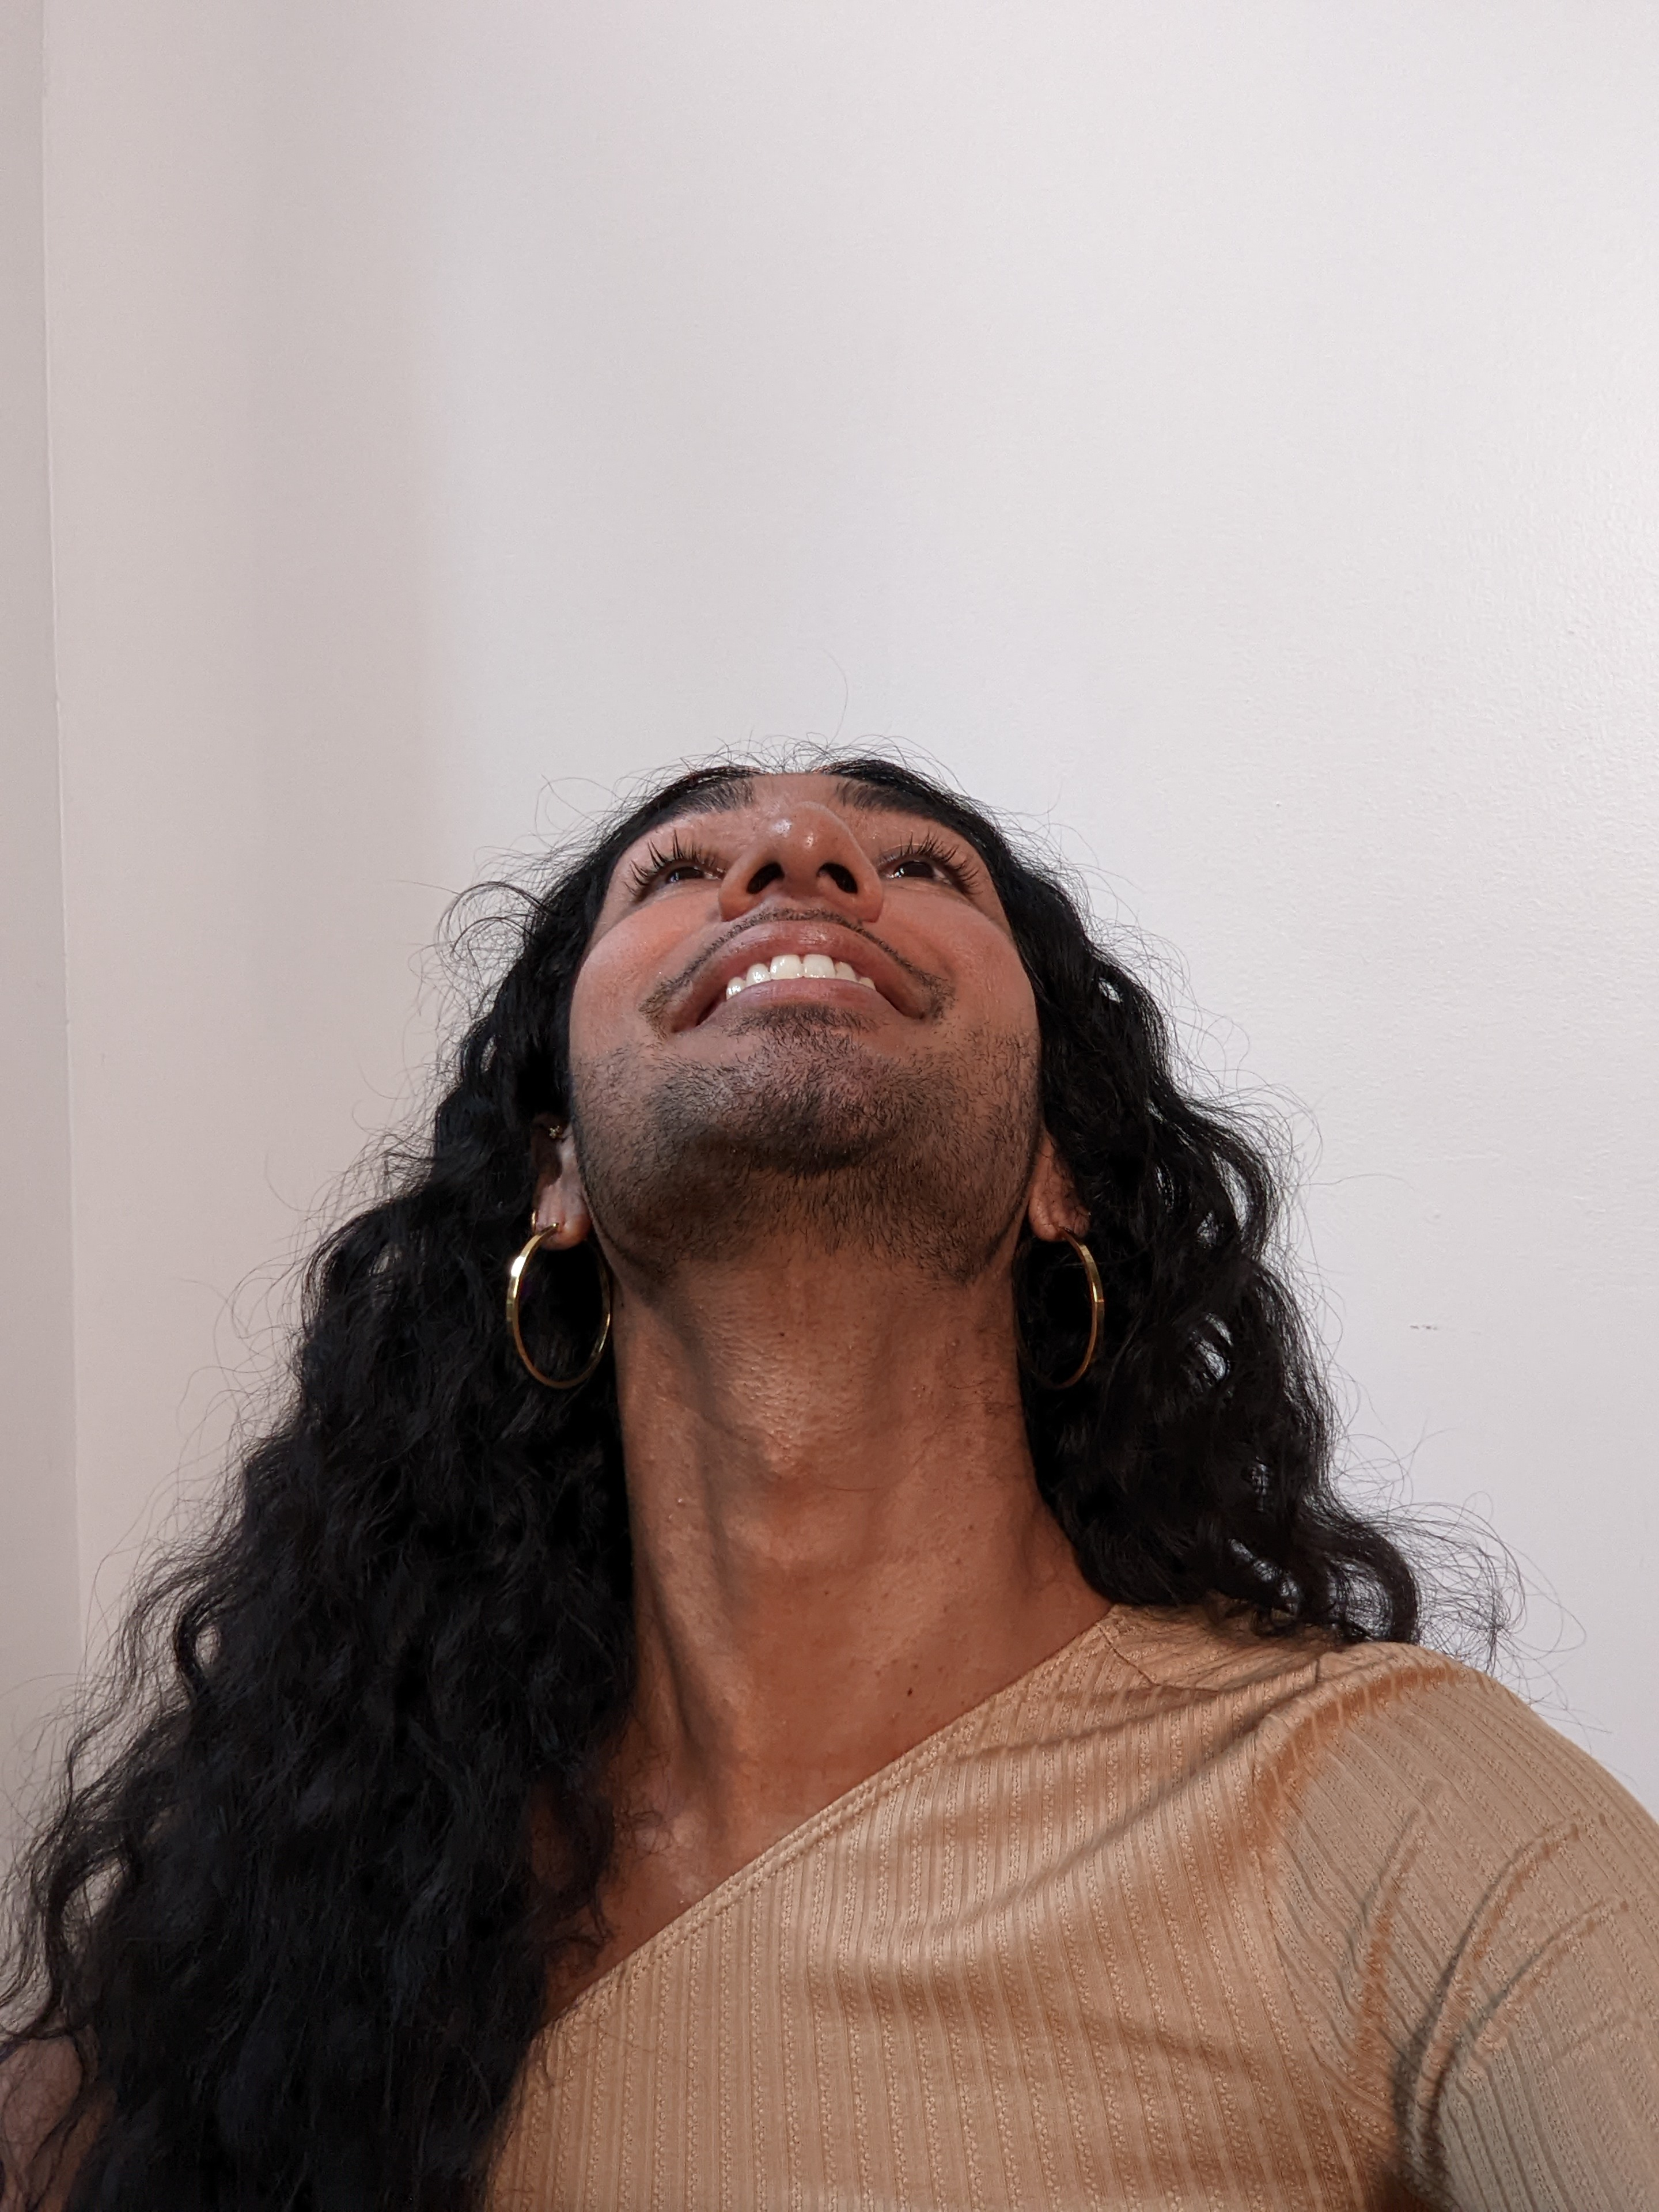
\includegraphics[height=10cm]{Template_Latex_TCC-UNIFTEC/_lib/imagens/bottom.jpg}\\ \centering\textbf{ a) Pose \textit{Bottom}}
    \label{fig: bottom}
    \end{minipage}
    \begin{minipage}[!]{0.55\linewidth}
    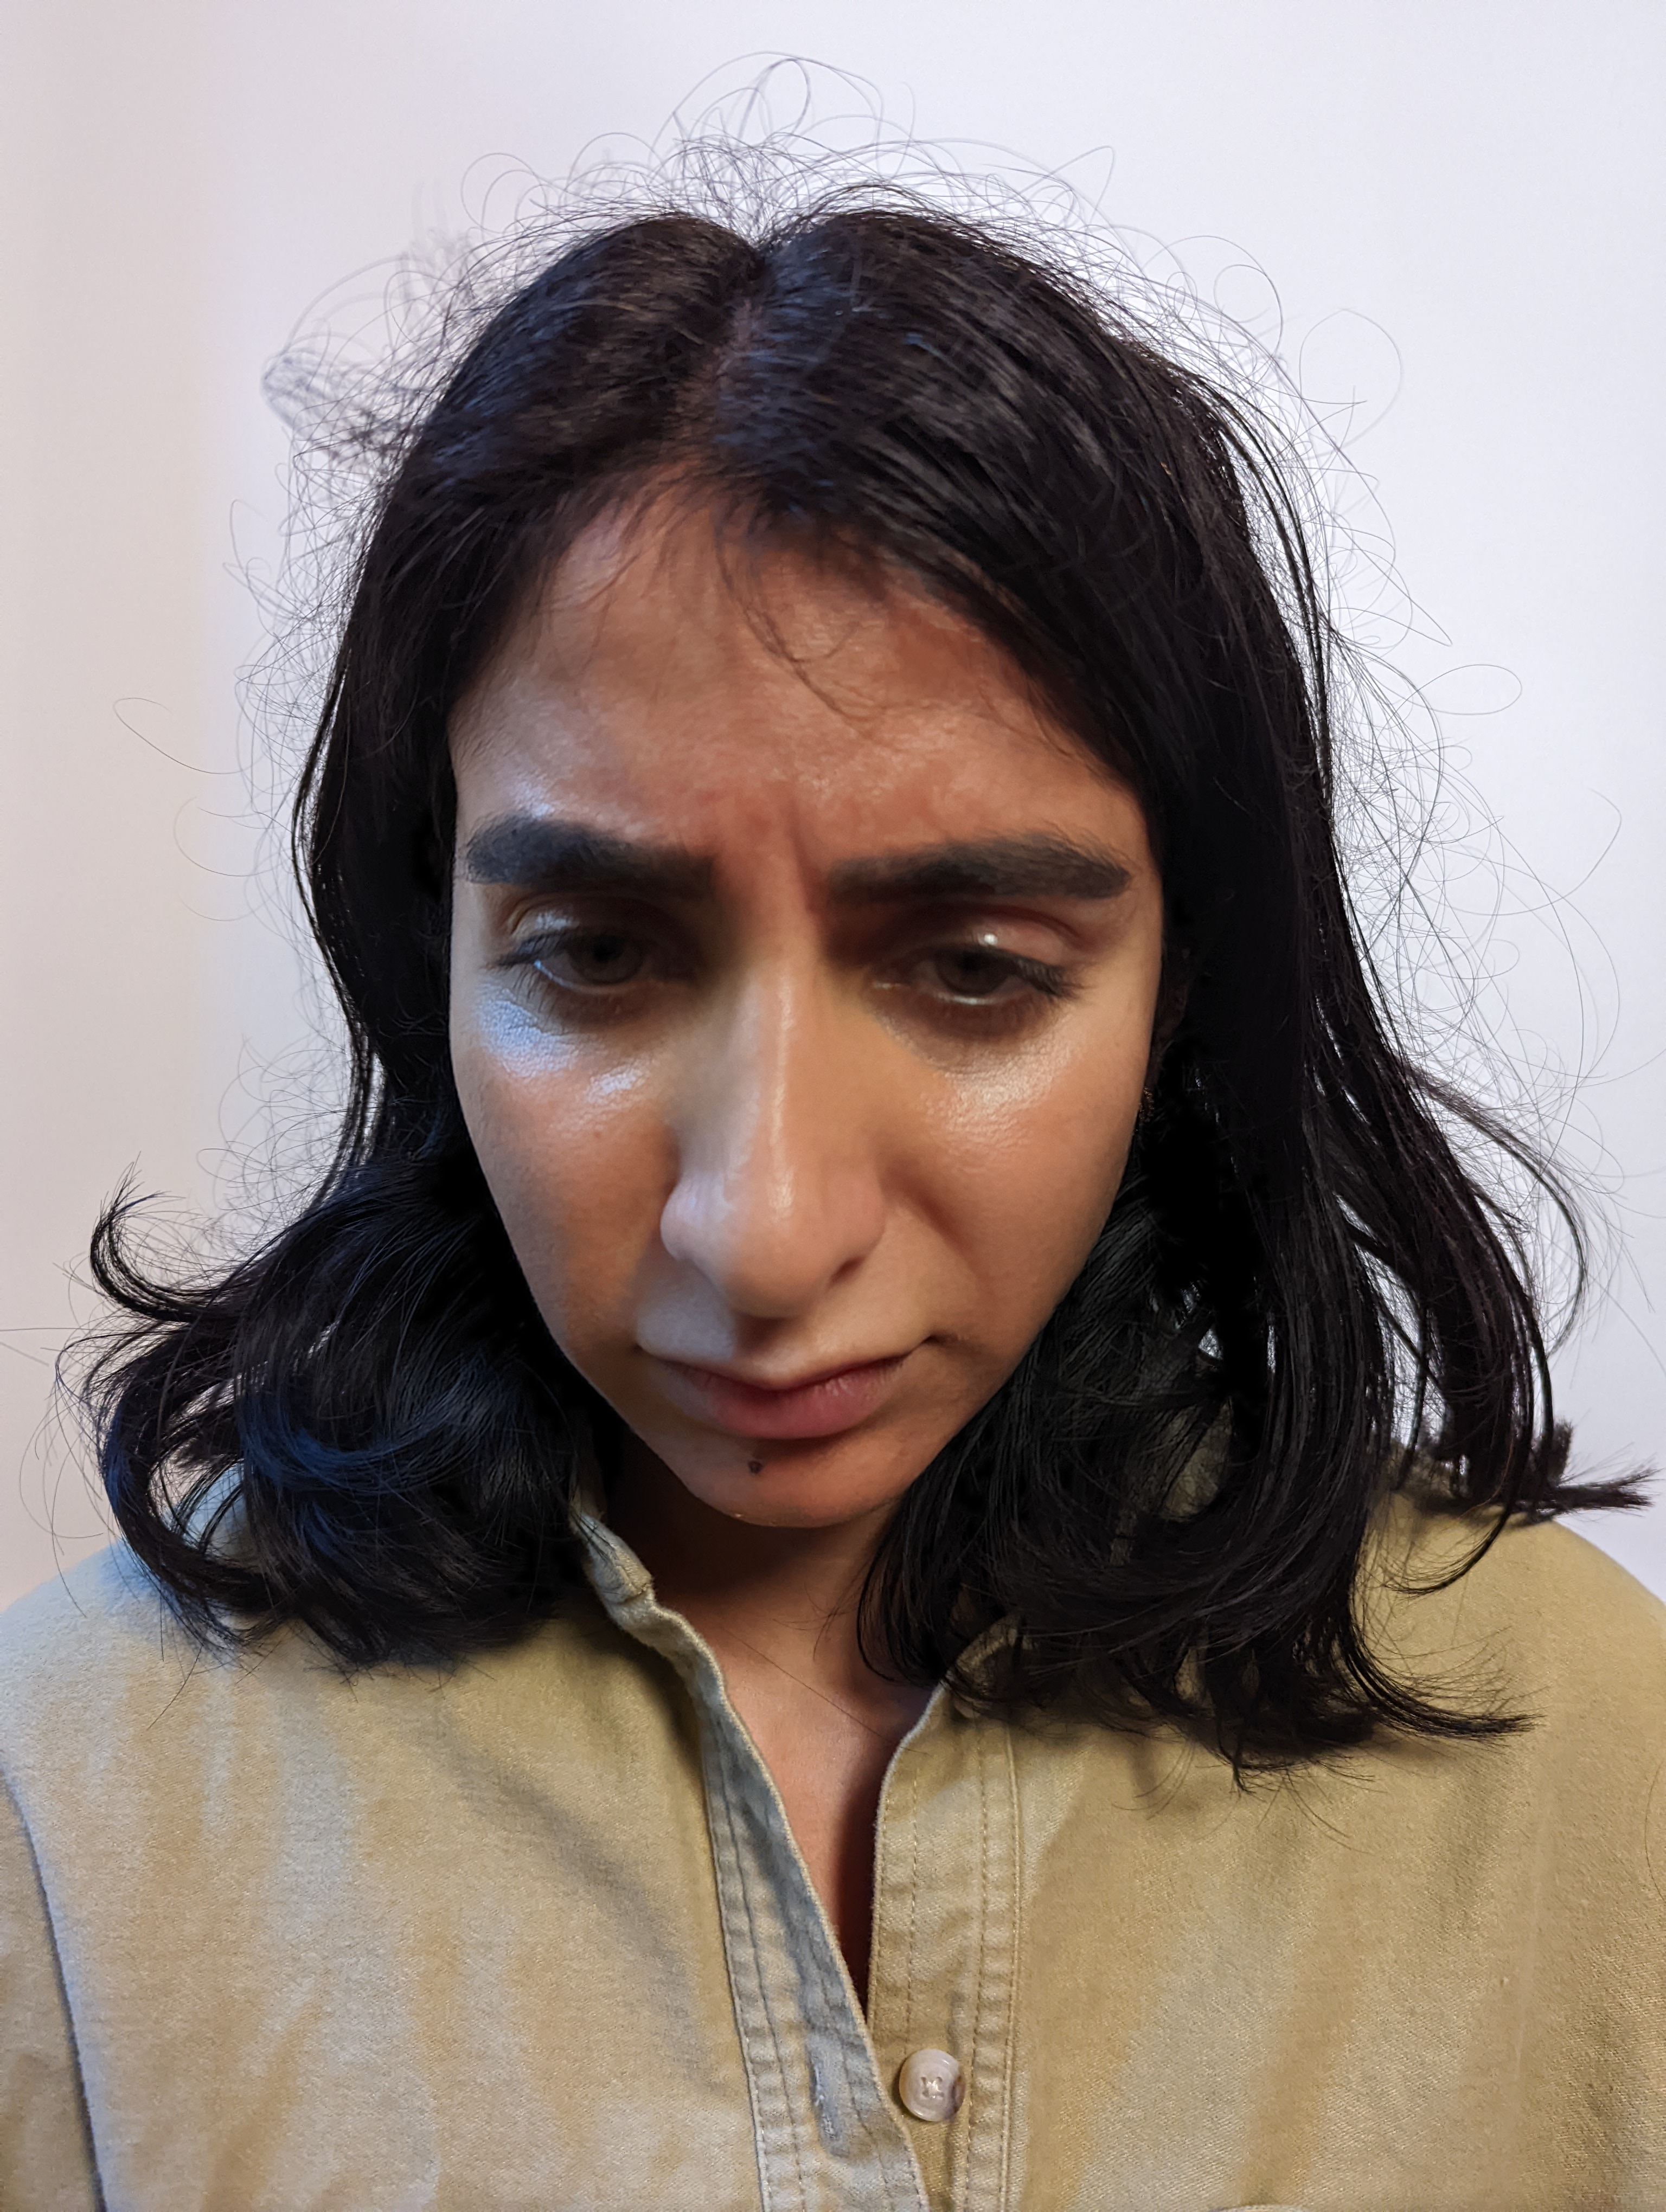
\includegraphics[height=10cm]{Template_Latex_TCC-UNIFTEC/_lib/imagens/frontal.jpg}\\ \centering\textbf{ b) Pose \textit{Frontal}}
    \label{fig: frontal}
    \end{minipage}
    \begin{minipage}[!]{0.55\linewidth}
    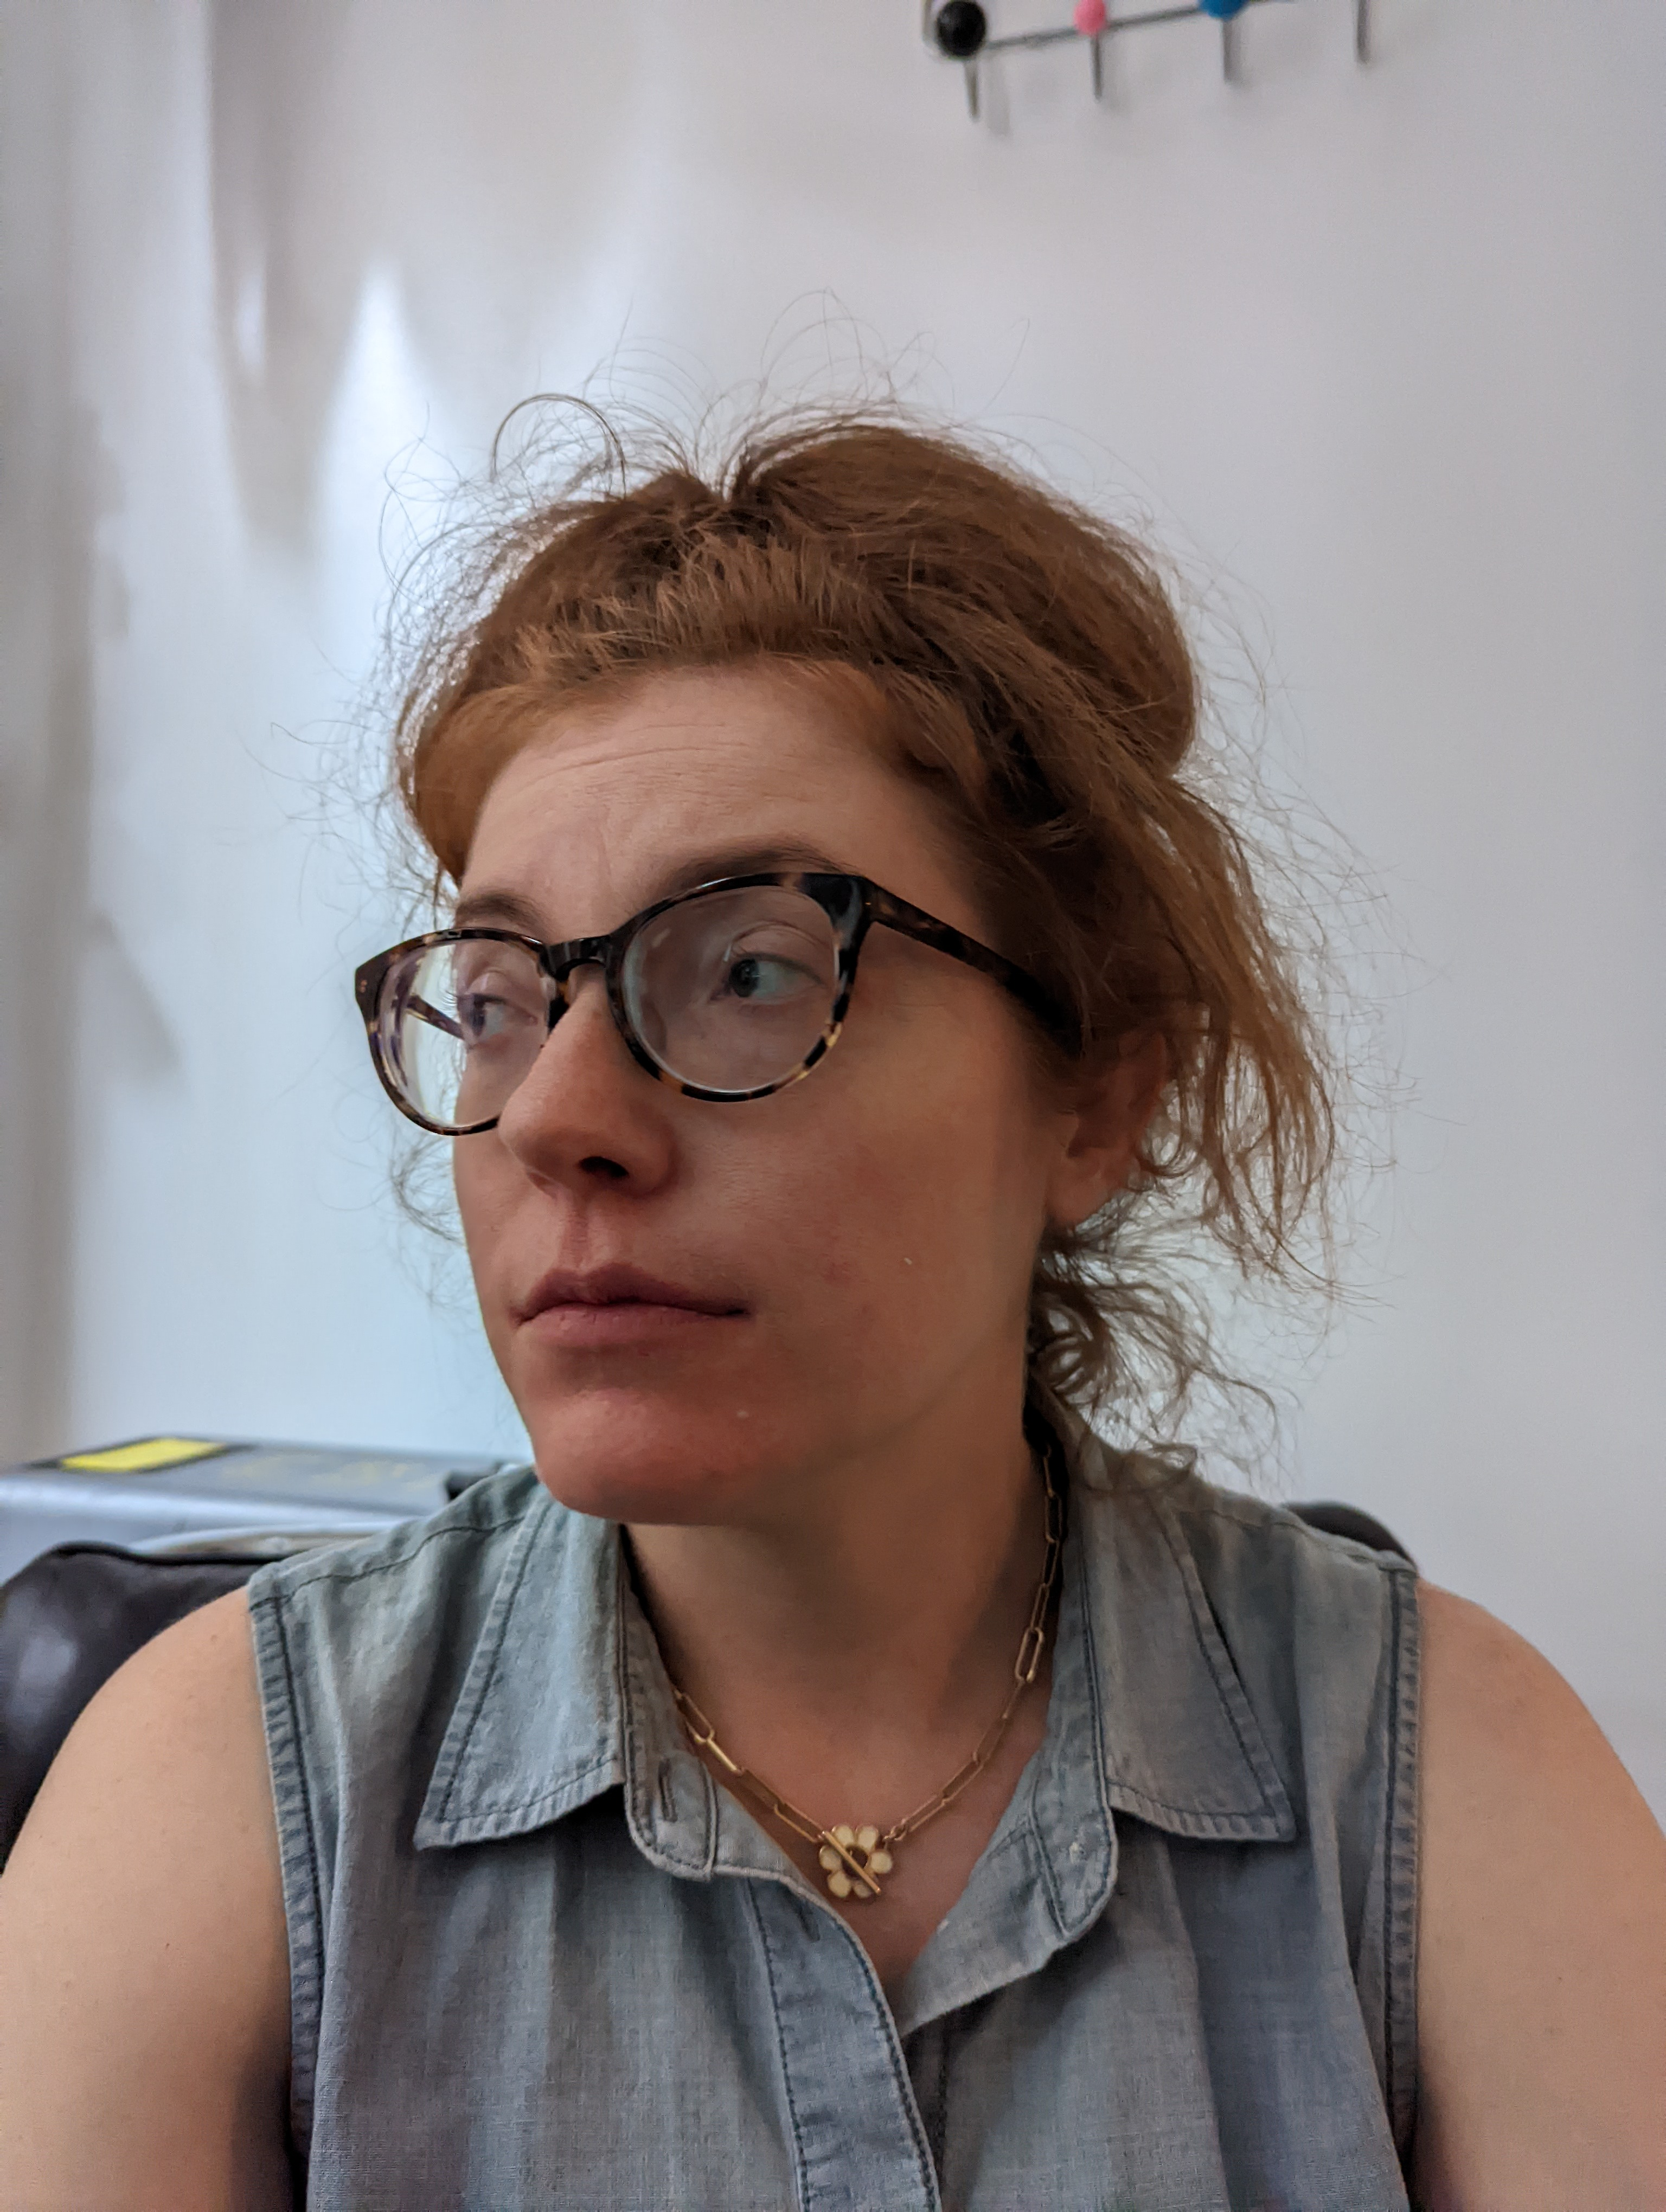
\includegraphics[height=10cm]{Template_Latex_TCC-UNIFTEC/_lib/imagens/side.jpg}\\ \centering\textbf{ c) Pose \textit{Side}}
    \label{fig: side}
    \end{minipage}
    \begin{minipage}[!]{0.55\linewidth}
    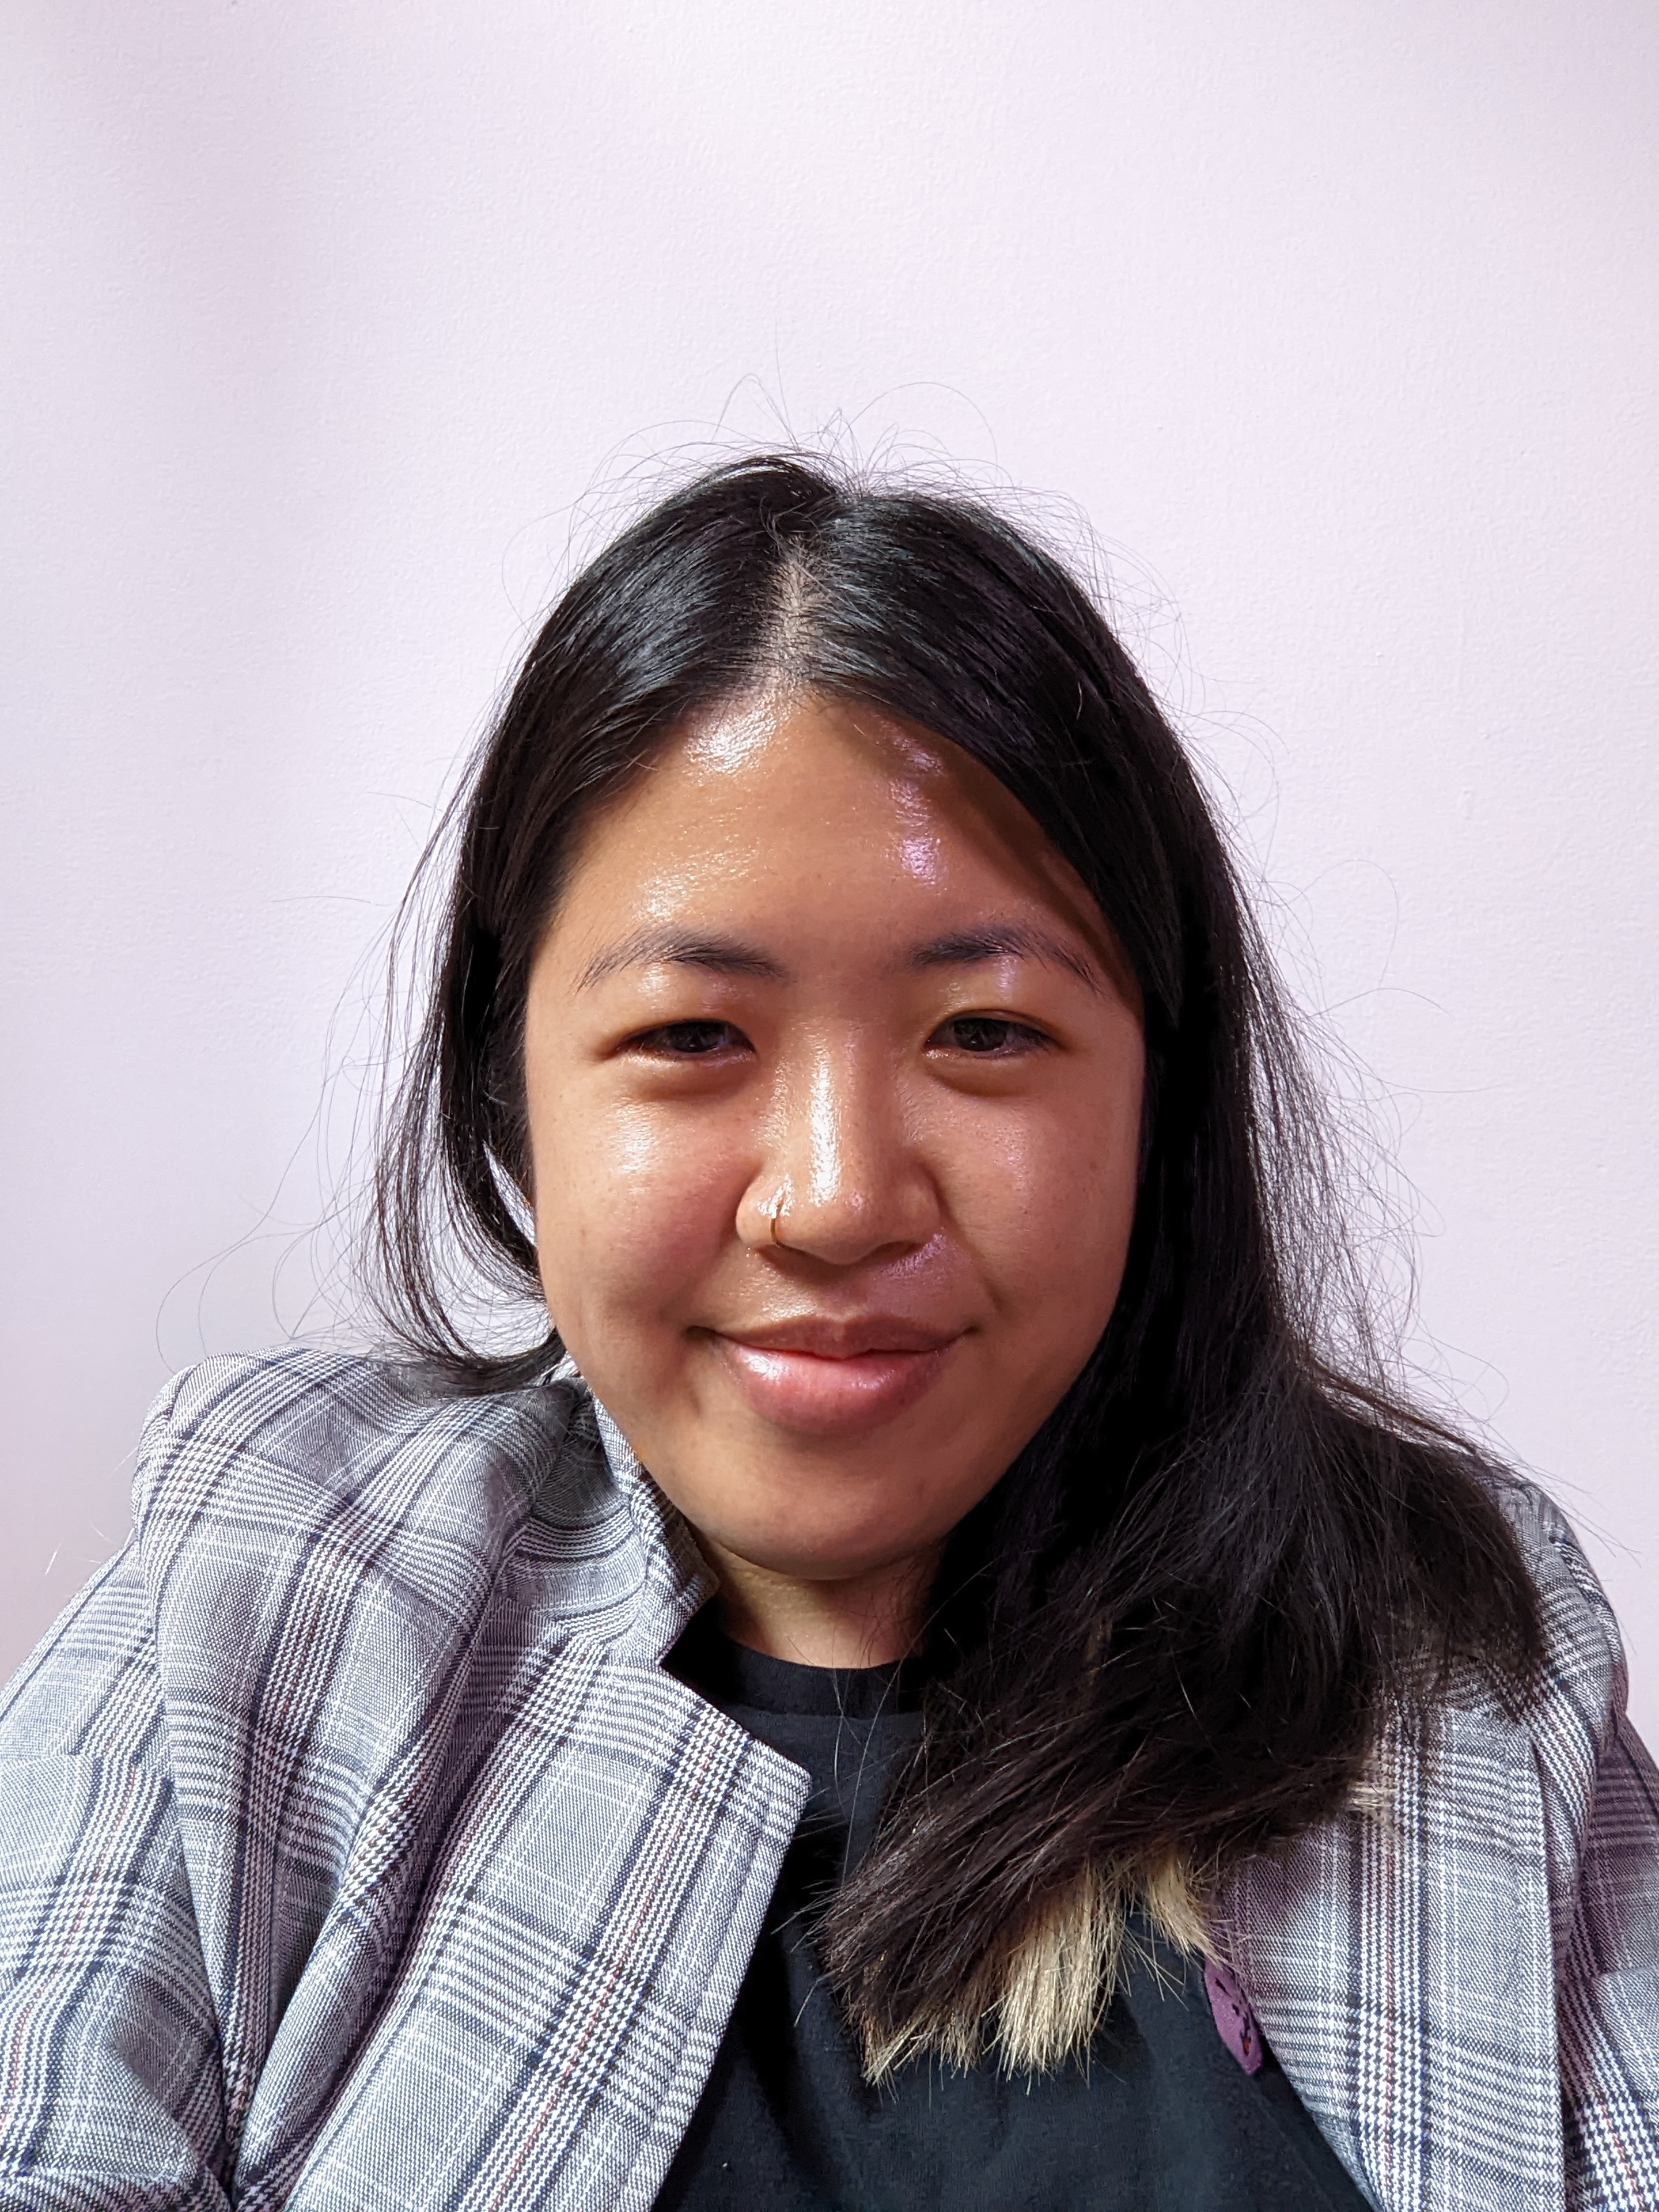
\includegraphics[height=10cm]{Template_Latex_TCC-UNIFTEC/_lib/imagens/facing_camera.jpg}\\ \centering\textbf{ d) Pose\textit{ Facing Camera}}
    \label{fig: facing_camera}
    \end{minipage}
\Fonte{Skin Tone Research} \footnote{https://skintone.google/mste-dataset}
\end{figure}

O \textit{dataset} MST-E possui 1515 imagens com diferentes poses e iluminações nas imagens. Sendo classificadas as poses como \textit{frontal} para pose de frente a câmera como na Figura \ref{fig: frontal}, \textit{bottom} para pose de frente com o queixo para cima como na Figura \ref{fig: bottom}, \textit{side} para pose com o rosto de lado, tanto para lado direito quanto para o lado esquerdo, como na Figura \ref{fig: side} e\textit{facing\_camera} para poses de frente olhando para a câmera como na Figura \ref{fig: facing_camera}, como pode ser visto na Figura \ref{fig: poses}. A quantidade de poses são relativas à escolha dos voluntários, assim como a presença de caretas. Quanto a iluminação, não há parametrização de quão claro ou escura é a iluminação utilizada. Há a classificação de duas diferentes iluminações, sendo elas \textit{poorly\_lit}, para iluminações de baixa qualidade,  e \textit{well\_lit}, para iluminações de boa qualidade. Não há padronização de plano de fundo nas fotos, visto que algumas imagens foram fotografadas ao ar livre. Algumas pessoas utilizam acessórios como máscaras e óculos. As imagens com máscara também foram categorizadas e separadas. Além disso, as imagens são catalogadas por Monk fornecendo os tons de pele verdadeiros do MST.


Para o propósito do trabalho desconsideraram-se os vídeos e as imagens com pessoas utilizando máscara e em pose não frontal. Para isso foi desenvolvido uma automatização como na Figura \ref{fig:x Visual_basic} para excluir os itens não necessários considerando as classificações compartilhadas na documentação do \textit{dataset}. 

\begin{figure}[h!]
\centering
\caption{Desenvolvimento para seleção de imagens relevantes}
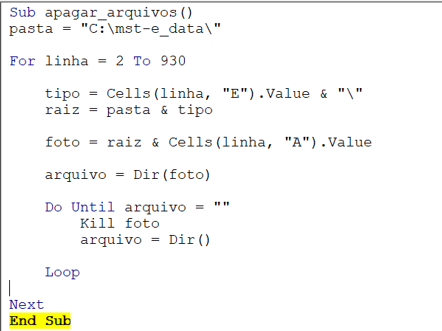
\includegraphics[scale=0.9]{Template_Latex_TCC-UNIFTEC/_lib/imagens/VisualBasic.png}

\label{fig:x Visual_basic}
\centering{\Fonte{Autor}}
\end{figure}

No desenvolvimento demonstrado na Figura \ref{fig:x Visual_basic}, é feito a leitura do arquivo csv disponibilizado pelo arquivo do \textit{dataset} MST-E. O arquivo foi modificado para ter somente as imagens a serem excluídas. No desenvolviwnto é verificao o nome das imagens disponibilizados no arquivo e procurados na pasta informada. O arquivo achado é excluído da pasta. O mesmo processo ocorre até a leitura do csv finalizar.

A partir disso, foi excluído os conteúdos de video e as imagens categorizadas com pose \textit{bottom} e \textit{side}, além das que continham máscara, mantendo as poses \textit{facing\_camera} e \textit{frontal} sem as fotos com máscara. Com isso, foram retiradas 929 arquivos, sendo elas imagens e vídeos não relevantes, totalizando em 617 imagens para estudo. Além disso, 32 imagens foram retiradas por estarem desfocadas e não serem viáveis de avaliação.

\subsection{Ajuste do tamanho da imagem}
Como as imagens possuíam tamanhos diferentes, para deixá-las todas em tamanho padrão utilizou-se a biblioteca OpenCV e o método resize(). O método pretende de redimensionar as imagens na altura, largura e interpolação com liberdade. No desenvolvimento, foi utilizado para ajustar a altura das imagens para 250px e largura para 250px. 

\subsection{Conversão de cores}
Para utilizar algumas funções do OpenCV e ter resultados mais precisos se faz necessário converter as cores das imagens ao longo do processamento. Ao longo do desenvolvimento foram realizadas ao todo 11 conversões de cores nas imagens. Para isso foi utilizada a função cvtColor()\footnote{https://docs.opencv.org/3.4/d8/d01/group__imgproc__color__conversions.html} que possui inúmeras possibilidades de conversão de cores. Cada modelo tem seu cálculo implícito, dependendo do parâmetro utilizado para conversão, mas para a conversão basta a inserção da imagem na função e o parâmetro que define qual sistema de cor está a imagem e para qual sistema deve-se ser convertido. Converteram-se as imagens do modelo de cor BGR para GRAY, BGR para HSV, HSV para BGR, BGR para RGB e BGR para LAB.

Como as imagens inseridas são lidas como BGR e não RGB todas as conversões de imagens partiram de BGR para os modelos de cor utilizados. Assim como para melhor visualização, visto que uma imagem em BGR não apresenta a visualização de cores esperadas originalmente.

Converteram-se as imagens dos modelos BGR para GRAY, para leitura e identificação de características. O modelo GRAY se refere a conversão para tons de cinza. A conversão foi utilizada para seguir o processo de pré-processamento de imagem que requer que a cor esteja em GRAY.

A conversão do sistema de cor BGR para HSV foi necessária para a extração de pele realizada com \textit{threshold} que será descrita ao longo do Capítulo \ref{cap:desenvolvimento}. Assim como a conversão do sistema de cor HSV para BGR para seguir o processo e visualização da imagem durante o desenvolvimento. 

Com relação à conversão do sistema de cor de BGR para LAB foi utilizada para a etapa de validação, onde os resultados foram calculados utilizando valores no modelo CIELab,  será descrita ao longo do Capítulo \ref{cap:desenvolvimento}.


\section{Pré-Processamento de Imagens}
O pré-processamento que se baseia em realizar identificações que facilitam a identificação das áreas relevantes, como a identificação de contornos, bordas e regiões da face como olhos, boca e nariz. Para isso é necessário o desenvolvimento de algumas etapas que serão abordadas ao longo desta seção.

\subsection{Remoção de regiões}
Com a imagem em GRAY, utilizou-se o método CascadeClassifier() para classificação em cascata da OpenCV. Primeiro ,o método CascadeClassifier é criado e o arquivo XML é carregado usando o método CascadeClassifier::load. Posteriormente, a detecção é feita usando o método CascadeClassifier::detectMultiScale, que retorna retângulos de limite para os rostos, boca, nariz ou olhos detectados. 
Para a identificação de regiões, utilizou-se dois arquivos do tipo XML da hospedagem oficial do OpenCV no repositório do GitHub\footnote{https://github.com/kipr/opencv/tree/master/data/haarcascades} modelados para a detecção frontal de face\footnote{https://github.com/kipr/opencv/blob/master/data/haarcascades/haarcascade\_frontalface\_default.xml} e detecção de olhos\footnote{https://github.com/kipr/opencv/blob/master/data/haarcascades/haarcascade\_eye.xml} e dois arquivos do tipo XML para a modelagem de detecção de nariz\footnote{https://github.com/atduskgreg/opencv\-processing/blob/master/lib/cascade\-files/haarcascade\_mcs\_nose.xml} e boca\footnote{https://github.com/atduskgreg/opencv\-processing/blob/master/lib/cascade\-files/haarcascade\_mcs\_mouth.xml} disponibilizados pela comunidade pelo repositório do GitHub \footnote{https://github.com/atduskgreg/opencv\-processing/tree/master/lib/cascade\-files}.
A identificação da face foi utilizada para identificar as faces e remover áreas de não interesse das outras análises. Para as regiões de olhos, boca e nariz, as áreas identificadas 
são pintadas da cor preta para serem desconsideradas, conforme Figura \ref{fig: Etapas_de_teste_roi}.

\begin{figure}[h]
\centering
\caption{Retirada de áreas de influência.(1) Imagem de referência; (2) Imagem de primeiro recorte;  (3) Imagem de exclusão de olhos; (4) Imagem de exclusão de nariz; e, (5) Imagem de exclusão de boca.}
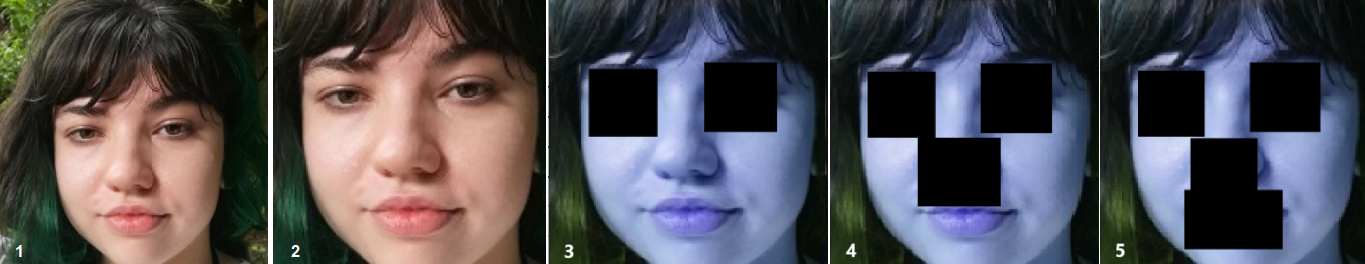
\includegraphics[scale=0.65]{Template_Latex_TCC-UNIFTEC/_lib/imagens/vittoriatestes2.png}

\label{fig: Etapas_de_teste_roi}
\centering{\Fonte{Autor}}
\end{figure}

Na Figura \ref{fig: Etapas_de_teste_roi} (1) demonstra-se a imagem sem tratamento colocado pelo usuário como referência, em seguida a imagem (2) onde é estabelecido o primeiro recorte da identificação do rosto pelo Haar Cascade. Na imagem (3) demonstra-se a exclusão da área dos olhos, por consequência a imagem (4) com a exclusão da região dos olhos e nariz e, por fim, a imagem (5) a exclusão da região dos, olhos, nariz e boca. 
A saída da função é a imagem  em BGR recortada e com as áreas de não interesse excluídas. A imagem então é convertida do modelo BGR para HSV para a extração de pixel de pele e não-pele.

\subsection{Segmentação de pele}

Para a segmentação de pele utiliza-se a função de extração de pele com \textit{threshold}. Para esse processo, cria-se uma imagem binária filtrando pixels com base em um limite definido no espaço de cor HSV. Cada pixel de uma imagem é verificado na faixa de limite, onde os valores limites são os valores HSV que denotam a faixa de tom de pele. O limite mínimo usado se enquadra no \textit{array} de 0, 48, 80 e o limite máximo se enquadra no \textit{array} 20, 255, 255. Para isso utilizou-se o método inRange() da biblioteca OpenCv para fazer a limitação, onde se o pixel lido estiver na faixa dos mínimos, torna-se o branco, se não, preto.

Em seguida, é utilizado o método GaussianBlur() da biblioteca OpenCV para suavização do resultado. Neste método é utilizado um kernel gaussiano e para isso especifica-se os valores de largura e altura do kernel. Também deve-se especificar o desvio padrão nas direções X e Y, sigmaX e sigmaY respectivamente. O desfoque gaussiano visa retirar o ruído da imagem, sendo uma variação dos valores nos níveis de cinza dos pixels na imagem, causados por erros na transmissão de dados, ou eventuais distorções causadas na fase de aquisição de uma imagem em geral. A função é dada como altamente eficaz na remoção do ruído gaussiano de uma imagem, por este motivo foi utilizado. Para isso, os parâmetros utilizados foram o resultado da imagem criada a partir do processamento de \textit{threshold}, valor de X e Y como 0, sendo os valores calculados a partir dos valores de sigma colocados, valores de 3 de sigmaX e sigmaY e borda padrão como 0.

Após a suavização, utilizando da biblioteca OpenCV, é executado o método bitwise\_and(). O método tem como objetivo obter a imagem final subtraída da imagem binária, resultando na imagem final convertida do espaço de cor HSV para BGR. O método bitwise\_and() visa a extração bit a bit de qualquer parte de uma imagem. E neste caso, utiliza-se o método para remover os pixel pretos tendo como parâmetros as imagens sem tratamento e a imagem gerada a partir do filtro de Gaussiana, tendo como resultado imagens como a Figura \ref{fig: Etapas_threshoding}. 

\begin{figure}[h]
\centering
\caption{Etapas de desenvolvimento. (1) Imagem de referência; (2) Imagem com recorte na face; e, (3) Remoção de pixel com Thresholding}
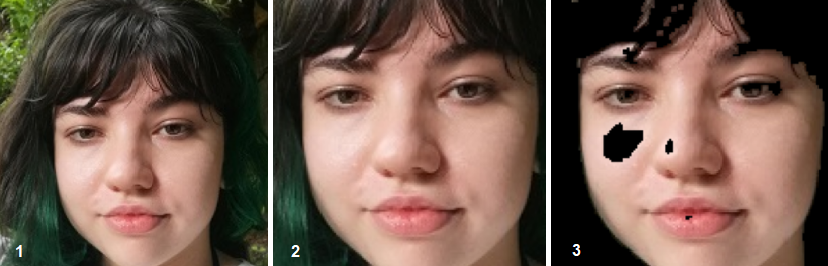
\includegraphics{Template_Latex_TCC-UNIFTEC/_lib/imagens/vittoriatestes.png}

\label{fig: Etapas_threshoding}
\centering{\Fonte{Autor}}
\end{figure}

A Figura \ref{fig: Etapas_threshoding} representa o resultado do processo de \textit{thresholding} isoladamente para melhor visualização. Nela foram ignorados a análise resultante utilizando a extração de regiões para representar apenas o resultado do processo de \textit{thresholding}. A imagem 1 representa a entrada original da imagem no sistema, a imagem 2 representa o recorte da imagem localizando a face e a imagem 3 o resultado das três etapas de \textit{ threshold} sendo limitação, suavização, subtração da imagem binária, demostrados todos no espaço RGB. Contudo, como saída do desenvolvimento da segmentação de pele temos uma imagem HSV que passa pela conversão para BGR.

\subsection{Seleção da cor dominante}
A extração de cores é executada utilizando o método Kmeans. O desenvolvimento utiliza uma cópia da imagem que está sendo a analisada e converte de BGR para RGB. A imagem convertida é reorganizada utilizando o método reshape(). O método reshape() tem o papel de mudar o formato do \textit{array} sem mudar o conteúdo
O método Kmeans verifica uma imagem no sistema de cor RGB e tem como parâmetro a quantidade de \textit{clusters} utilizados, a  geração de números aleatórios para inicialização do centroide como nulo e o número de vezes que o algoritmo k-means é executado com centroides diferentes, determinado como automático.

Após a extração de cores seleciona-se a cor dominante com a verificação de pixel por pixel. A quantidade de ocorrência de cores é verificada, sendo somado a quantidade de pixels da mesma cor. As cores mais comuns encontradas são reorganizadas em sequência crescente de quantidade ocorrência para identificação da cor mais dominante.Além de ser efetuado o cálculo de percentagem relativa a sua proporção.

 
\section{Resultado visual}
Para fins visuais é criada uma barra de cores para visualização das cores dominantes encontradas. As cores analisadas com as suas respectivas percentagens são adicionadas em um \textit{array}. Os valores de porcentagem são organizados de forma decrescente. Sendo, a primeira cor, a esquerda, adicionada na barra, a cor com a maior porcentagem. Por consequência, a cor mais dominante. Criando-se a imagem com as respectivas cores encontradas e a demonstração visual da quantidade percentual encontrada, conforme Figura \ref{fig:x Paleta_resultante}.  

\begin{figure}[h]
\centering
\caption{Paleta resultante}

\includegraphics{Template_Latex_TCC-UNIFTEC/_lib/imagens/paleta.png}

\label{fig:x Paleta_resultante}
\centering{\Fonte{Autor}}
\end{figure}


\section{Validação}
Para validação de resultados comparou-se os valores categorizados por Monk aos resultados alcançados pelo desenvolvimento. Utilizando a biblioteca Scikit-image e o método deltaE\_ciede2000(). O método baseia-se em comparar duas cores no sistema de cor CIELab. Para isso foi feita a conversão do sistema de cor BGR para Lab.

No desenvolvimento, utilizou-se os 10 tons da paleta de Monk disponibilizados no modelo CIELab presentes da documentação da paleta\footnote{https://skintone.google/get-started}. O método requer a inserção de duas várias com o valor de cor CIELab, fator de luminosidade (kL), fator de cromaticidade (kC), fator de escala de matiz (kH) e de canais com valores padrões. No desenvolvimento utilizou como referência a cor disponibilizada pela paleta de Monk e a cor de comparação a cor dominante encontrada. Os demais parâmetros utilizaram do valor padrão igual a 1

Se realizaram três analises diferentes e os resultados foram salvos na planilha csv criada. Na primeira análise é realizada o cálculo CIEDE2000 para todos os tons de MST. Nisso a análise baseia-se na comparação de valores das 10 cores MST com a cor dominante, sendo os 10 valores salvos em uma lista. Esses valores são analisados e verificados com o método min() para trazer o valor de distância mínima, sendo o valor ideal esperado de todos os valores que constam na lista, sendo salvo no arquivo csv como mínimo\_lab. 

A segunda análise se baseia em selecionar o valor de categorização MST conforme o valor mínimo encontrado. Para isso utiliza-se o método index() para selecionar a posição na lista em que se encontra o valor mínimo encontrado anteriormente. Este valor é salvo no arquivo csv como classificacao\_indicada\_lab. Para a terceira análise, utilizando a cor classificada por Monk e a cor dominante encontrada, se refaz o cálculo com o método deltaE\_ciede2000() para calcular o valor verdadeiro de acordo com Monk. Ou seja, é apenas avaliado a cor classificada por Monk e a cor encontrada tendo como resultado a distância a qual não é necessariamente a menor entre todas as cores, sendo este valor salvo no arquivo csv como distancia\_lab.

Em conclusão é feito o cálculo de acurácia conforme realizado no artigo \cite{Classification_Algorithm_for_Skin_Color_CASCo_A_new_tool} . O cálculo de baseia em subtrair de 100 o valor de minimo\_lab. 

Após o processamento, salvam-se as informações de nome de arquivo, pose, característica de iluminação, tom MST, o tom encontrado em CIELab, a distância mínima ideal, a distância encontrada e a acurácia em um arquivo do tipo csv.

Criação de arquivo csv para estudo e comparação de resultados. Cada imagem analisada tem seus dados salvos para verificação dos resultados em um arquivo criado durante o processamento. Como as imagens do \textit{dataset} já foram categorizadas por Dr. Monk as informações que constam no de nome da imagem apenas para referência, número de objeto estudado, pose utilizada, descrição de luz e a classificação mst são extraídos e salvos no arquivo csv. Além disso, são adicionadas as informações CIELab do tom MST e os valores resultantes do desenvolvimento como a cor dominante em CIELab, a menor distância calculada encontrada entre todas as cores da paleta para CIELab, a distância resultante encontrada entre a cor dominante CIELAB e o tom classificado, a classificação indicada conforme a distância resultante e a acurácia.

A criação do arquivo se dá com a função open() da biblioteca CSV. A função permite criação, escrita, leitura e modificação de arquivo. No desenvolvimento foi utilizada a função open() para criar o arquivo local  como o modo 'w' e modificá-lo como o modo 'a'.

O método DictWriter() foi utilizado para criar o cabeçalho com as informações \textit{'image\_name', 'subject','pose', 'light', 'MST','LAB','distancia_lab', 'minimo\_lab', 'classificacao_indicada_lab', 'acuracia'} e seu demilitado sendo uma vírgula. Para adicioná-lo ao arquivo criado utilizou-se o método writerheader() para adicioná-lo ao arquivo.

Para a modificação do arquivo csv, o arquivo é reaberto para modificação e com o método writer() e writerow() é adicionado uma nova linha ao arquivo à cada imagem processada.

% \section{Considerações finais}